
\documentclass{article}

% ------------------------------------------------------------------
% ICLR 2027 style.
% Place the official iclr2027_conference.sty and .bst files next to
% this source before submission. The fallback branch allows this draft
% to compile before those files are copied into the project.
% ------------------------------------------------------------------
\newif\ificlrstyle
\IfFileExists{iclr2027_conference.sty}{
  \iclrstyletrue
  \usepackage{iclr2027_conference,times}
}{
  \iclrstylefalse
  \usepackage[letterpaper,textwidth=5.5in,textheight=9in,centering]{geometry}
  \usepackage{times}
  \usepackage[authoryear,round]{natbib}
  \pagestyle{plain}
}
\providecommand{\iclrfinalcopy}{}
% \iclrfinalcopy  % Uncomment only for the camera-ready version.

\usepackage[T1]{fontenc}
\usepackage{microtype}
\usepackage{amsmath,amssymb,amsthm,mathtools,bm}
\usepackage{booktabs,tabularx,array,multirow}
\usepackage{graphicx}
\usepackage{xcolor}
\usepackage{enumitem}
\usepackage{caption}
\usepackage{subcaption}
\usepackage{algorithm}
\usepackage[noend]{algpseudocode}
\usepackage{tikz}
\usetikzlibrary{arrows.meta,positioning,fit,calc,backgrounds}
\usepackage{xurl}
\usepackage{hyperref}
\usepackage[nameinlink,capitalise,noabbrev]{cleveref}

% ------------------------------------------------------------------
% Draft controls.
% ------------------------------------------------------------------
\definecolor{placeholderred}{RGB}{170,35,45}
\definecolor{methodblue}{RGB}{35,87,137}
\definecolor{methodteal}{RGB}{30,125,112}
\definecolor{softgray}{RGB}{244,246,248}
\definecolor{darkgray}{RGB}{70,76,82}

\newcommand{\TBD}{\textcolor{placeholderred}{\textbf{TBD}}}
\newcommand{\resultplaceholder}[1]{%
  \par\noindent{\small\textcolor{placeholderred}{%
  \textbf{RESULT PLACEHOLDER.} #1}}\par}
\newcommand{\dataplaceholder}[1]{%
  \textcolor{placeholderred}{\textbf{[DATA CHECK: #1]}}}
\newcommand{\figureplaceholder}[2][1.45in]{%
  \begin{center}
  \fcolorbox{placeholderred}{placeholderred!3}{%
    \begin{minipage}[c][#1][c]{0.92\linewidth}
    \centering\small\textcolor{placeholderred}{\textbf{EMPIRICAL FIGURE PLACEHOLDER}}\\[0.5em]
    \parbox{0.86\linewidth}{\centering #2}
    \end{minipage}}
  \end{center}}
\newcommand{\draftwarning}{%
  \begin{center}
  \fcolorbox{placeholderred}{placeholderred!4}{%
  \parbox{0.93\linewidth}{\centering\small\textcolor{placeholderred}{%
  \textbf{Draft status:} theory and experimental protocols are written;
  all red empirical placeholders must be replaced by verified results before submission.}}}
  \end{center}}

% ------------------------------------------------------------------
% Mathematics.
% ------------------------------------------------------------------
\newcommand{\R}{\mathbb R}
\newcommand{\E}{\mathbb E}
\newcommand{\Pp}{\mathbb P}
\newcommand{\KL}{\mathrm{KL}}
\newcommand{\TV}{d_{\mathrm{TV}}}
\newcommand{\Law}{\mathcal L}
\newcommand{\osc}{\operatorname{osc}}
\newcommand{\ess}{\mathrm{ESS}}
\newcommand{\Z}{\mathcal Z}
\newcommand{\Hist}{\mathcal H}
\newcommand{\PathP}{\mathbf P}
\newcommand{\PathQ}{\mathbf Q}
\newcommand{\PathR}{\mathbf R}
\newcommand{\eps}{\varepsilon}
\newcommand{\dd}{\,\mathrm d}
\newcommand{\ind}{\mathbbm 1}
\newcommand{\push}{_{\#}}
\DeclareMathOperator*{\argmin}{arg\,min}
\DeclareMathOperator{\Ber}{Ber}
\DeclareMathOperator{\Cov}{Cov}
\DeclareMathOperator{\Var}{Var}
\DeclareMathOperator{\diag}{diag}
\DeclareMathOperator{\softmax}{softmax}
\DeclareMathOperator{\sigmoid}{sigmoid}

\newtheorem{definition}{Definition}
\newtheorem{proposition}[definition]{Proposition}
\newtheorem{lemma}[definition]{Lemma}
\newtheorem{theorem}[definition]{Theorem}
\newtheorem{corollary}[definition]{Corollary}
\newtheorem{assumption}[definition]{Assumption}
\theoremstyle{remark}
\newtheorem{remark}[definition]{Remark}
\newtheorem{example}[definition]{Example}

\crefname{assumption}{assumption}{assumptions}
\Crefname{assumption}{Assumption}{Assumptions}

\title{Compatibility-Aware Path Responses for Learned Stochastic Dynamics}

\author{Anonymous authors}

\begin{document}
\maketitle
% \draftwarning  % Uncomment while editing if a title-page warning is useful.

\begin{abstract}
Learned transition models are often interrogated by editing one coordinate of a
recorded history and rolling the model forward. Such a query can evaluate the
model on histories with little or no observational support, so two generators
with essentially indistinguishable predictive fit may return incompatible
responses. We introduce a different, explicitly noncausal estimand:
a \emph{compatibility-aware repaired path response}. Candidate prefixes are
generated under the unchanged transition law, softly clamped at a source
statistic, selectively anchored to a factual episode, and reweighted only up to
a declared temporal cut. The future is then sampled without further weighting.
The construction returns a full future distribution together with a
compatibility mass that quantifies how much of the natural path law supports
the query.

We prove that the response is a unique functional of a declared finite-memory
path law, establish a finite-sample low-coverage barrier for local transition
queries, and derive finite-horizon robustness bounds that separate
compatibility-amplified pre-cut error from ordinary post-cut forecast error.
We show that inverse-compatibility amplification is unavoidable in general and
derive an oracle tradeoff between soft-clamp bias and generator error. A
sample-only sequential Monte Carlo algorithm implements the response for any
conditional generator that can produce next-state samples.
We evaluate the method on near-manifold dynamics, a mean-blind multistable
system, a constrained physical world model, controlled misspecification, and
whole-brain \emph{C.\ elegans} calcium recordings.
\resultplaceholder{Replace the final sentence with two concrete quantitative
findings: one controlled-oracle result and one externally validated neural
result.}
The proposed response does not by itself identify a physical intervention; it
provides a support-aware and diagnostically explicit way to ask finite
distributional questions of learned stochastic dynamics.
\end{abstract}

\section{Introduction}
\label{sec:intro}

A conditional generative model of dynamics can answer far more queries than a
single supervised predictor. Given a recent history, it can generate future
trajectories, estimate event probabilities, compare modes of behavior, and
support post-hoc scientific hypotheses. This flexibility also creates a
failure mode that is easy to overlook. A user may take a recorded history,
replace one neuron's activity, one physical coordinate, or one latent
component by a desired value, and roll the model forward while holding the
remaining coordinates fixed. The model will usually return a numerical
forecast. That answer need not be determined by the observational data.

The issue is not merely that the query is ``out of distribution'' in a vague
sense. Histories of a nonlinear system often satisfy geometric, dynamical, or
representational constraints. Editing one coordinate can break those
constraints while preserving all other coordinates. A conditional model is
only statistically constrained where histories occur; its continuation away
from that region can be selected by architecture, regularization, or
optimization rather than by data. Consequently, ordinary held-out likelihood
can be nearly unchanged while the hard-edit response varies substantially.

We replace the hard edit by a different question. Starting from a boundary
history, we generate complete alternative prefixes under the learned
transition law. We favor prefixes whose designated source statistic is near a
target value and whose selected contextual coordinates remain near the factual
episode. At the source-time cut, all weights are removed and each repaired
prefix is rolled forward under the original transition kernel. The resulting
contrast between target and baseline source values is a difference between
future \emph{laws}, not only means. We call it a
\emph{repaired path response}; ``repair'' changes the mixing law over naturally
generated prefixes and never surgically modifies a generated state.

\begin{figure}[t]
\centering
\resizebox{\linewidth}{!}{%
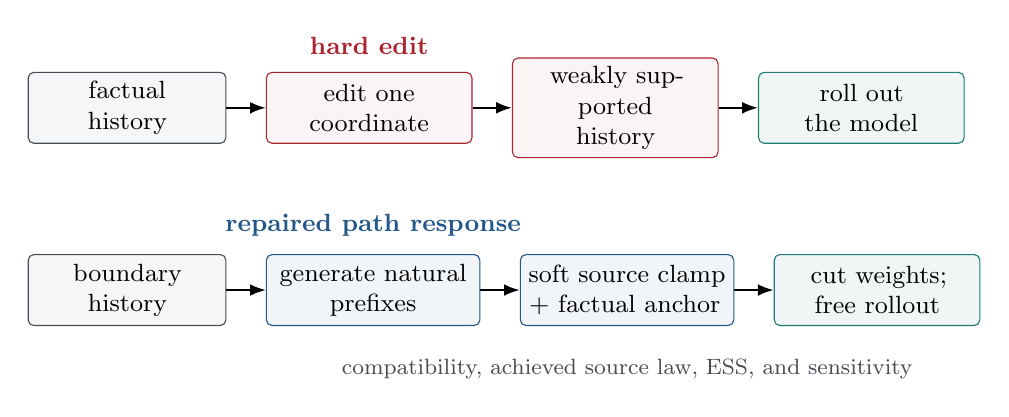
\begin{tikzpicture}[
  node distance=4mm and 5mm,
  every node/.style={font=\small,align=center},
  factual/.style={draw=darkgray,rounded corners=2pt,fill=softgray,
                  minimum height=9mm,text width=23mm,inner sep=3pt},
  bad/.style={draw=placeholderred,rounded corners=2pt,fill=placeholderred!5,
              minimum height=9mm,text width=24mm,inner sep=3pt},
  good/.style={draw=methodblue,rounded corners=2pt,fill=methodblue!6,
               minimum height=9mm,text width=25mm,inner sep=3pt},
  future/.style={draw=methodteal,rounded corners=2pt,fill=methodteal!7,
                 minimum height=9mm,text width=24mm,inner sep=3pt},
  arr/.style={-{Latex[length=2mm]},thick}
]
\node[factual] (fact1) {factual\\history};
\node[bad,right=of fact1] (edit) {edit one\\coordinate};
\node[bad,right=of edit] (off) {weakly supported\\history};
\node[future,right=of off] (roll1) {roll out\\the model};
\draw[arr] (fact1)--(edit);
\draw[arr] (edit)--(off);
\draw[arr] (off)--(roll1);
\node[above=1mm of edit,font=\bfseries\small,text=placeholderred] {hard edit};

\node[factual,below=14mm of fact1] (boundary) {boundary\\history};
\node[good,right=of boundary] (sample) {generate natural\\prefixes};
\node[good,right=of sample] (weight) {soft source clamp\\+ factual anchor};
\node[future,right=of weight] (roll2) {cut weights;\\free rollout};
\draw[arr] (boundary)--(sample);
\draw[arr] (sample)--(weight);
\draw[arr] (weight)--(roll2);
\node[above=1mm of sample,font=\bfseries\small,text=methodblue]
  {repaired path response};

\node[below=3mm of weight,font=\footnotesize,text=darkgray]
  {compatibility, achieved source law, ESS, and sensitivity};
\end{tikzpicture}}
\caption{A hard coordinate edit can expose an unconstrained extension of a
learned transition law. The proposed response instead reweights complete
prefixes generated by the model, stops all weighting at a temporal cut, and
then samples the future under the unchanged kernel.}
\label{fig:overview}
\end{figure}

The central diagnostic is \emph{compatibility}: the normalized mass of natural
prefixes selected by the source clamp and factual anchor. Compatibility has a
precise operational meaning as an acceptance probability. It also controls the
worst-case amplification of model error before the temporal cut. Low
compatibility therefore links statistical fragility, importance-weight
concentration, and the need to abstain. It is not, however, a certificate that
the learned model is biologically or physically correct.

Our contributions are:
\begin{enumerate}[leftmargin=1.5em]
  \item We formalize why hard history edits can be unidentifiable on null sets
  and statistically unrecoverable in low-coverage regions. A finite-sample
  lower bound shows that a local transition response on a region of mass \(p\)
  cannot be reliably learned when the effective sample size satisfies
  \(Np\ll 1\).
  \item We define an episode-anchored, cut-indexed distributional response for
  finite-memory transition laws. The source is softly clamped, selected
  factual coordinates are softly anchored, and the post-cut future kernel is
  exactly preserved.
  \item We derive response-specific robustness bounds. Pre-cut path error is
  amplified by inverse compatibility, whereas post-cut error accumulates as
  ordinary forecast error. A matching conditioning construction shows that
  inverse-compatibility dependence is unavoidable without stronger
  assumptions.
  \item We give a sample-only sequential Monte Carlo (SMC) implementation and
  an evaluation protocol that separates algorithm error, generator error, and
  the semantic gap to physical intervention. The real-data case study uses
  stimulus-aligned whole-brain \emph{C.\ elegans} activity and independent
  perturbational references.
\end{enumerate}

We do not claim a new exponential-tilting identity, bridge construction, or
particle algorithm. The contribution is the response object, its temporal and
diagnostic specialization to learned transition models, and the accompanying
stability and evaluation framework.

\section{Setup and the failure of hard history editing}
\label{sec:setup}

\subsection{Learned finite-memory dynamics}

Let \(X_t\in\R^d\) denote an observed state and let \(S_t\) denote an observed
exogenous context, such as a stimulus indicator. For a chosen history length
\(L\), define
\[
  \Hist_t=(X_{t-L+1},\ldots,X_t),\qquad
  \Sigma_t=(S_{t-L+1},\ldots,S_t).
\]
The order-\(L\) population transition kernel is
\begin{equation}
  P_t(h,\dd y)
  =\Law(X_{t+1}\mid \Hist_t=h,\Sigma_t),
  \label{eq:population-kernel}
\end{equation}
and a learned conditional generator supplies an approximation
\(Q_t(h,\dd y)\). We assume that \(Q_t\) can at least produce conditional
samples. Log densities or scores may be available but are not required.

The finite-memory kernel induces a Markov law on the augmented history state.
This induced law equals the biological or physical path law only under
\emph{predictive-state sufficiency},
\begin{equation}
  \Law(X_{t+1}\mid X_{-\infty:t},S_{-\infty:t})
  =
  \Law(X_{t+1}\mid \Hist_t,\Sigma_t)
  \quad\text{a.s.}
  \label{eq:predictive-sufficiency}
\end{equation}
Without \cref{eq:predictive-sufficiency}, our estimand remains a well-defined
response of the order-\(L\) predictive projection, but it need not equal a
response of the latent biological system.

Fix a factual prefix \(x^\star_{-B:0}\), relabel the source time as \(0\), and
hold the stimulus schedule fixed. Let
\(A(X_{-B:0})\in\R^{d_A}\) be a source statistic and let
\(T(X_{1:K})\) be a future statistic. A hard-edit query replaces selected
components of \(x^\star_0\) by a target \(a\) and rolls \(Q\) forward from the
edited history. This operation evaluates \(Q\) at a numerical history that may
have negligible probability under the observational history law.

\subsection{Null-set nonidentification}

The basic obstruction is visible in a redundant representation. Suppose the
observed state is \(X_t=(U_t,V_t)\) and genuine histories satisfy \(U_t=V_t\).
For any \(\beta\in\R\), define
\begin{equation}
  m_\beta(h)=m_0(h)+\beta(U_t-V_t).
  \label{eq:beta-extension}
\end{equation}
Every \(m_\beta\) agrees on all genuine histories, while the edit
\((u_0,u_0)\mapsto(u,u_0)\) changes the next-state prediction by
\(\beta(u-u_0)\).

\begin{proposition}[Hard-edit nonidentification]
\label{prop:hard-nonid}
Let \(H\) be the conditioning history with observational law \(P_H\). If an
edit maps factual histories to a measurable set \(C\) with \(P_H(C)=0\), and no
structural or continuity restriction fixes the conditional kernel on \(C\),
then the resulting hard-edit forecast is not a functional of the
observational joint law. Two regular conditional kernels can agree
\(P_H\)-almost surely and return arbitrarily different forecasts on \(C\).
\end{proposition}

This is a standard version-of-a-conditional-law fact. Its practical
consequence is less standard: a neural generator can always return a number,
even when the number is determined only by an off-support extension.

\subsection{A finite-sample low-coverage barrier}

Exact null sets are not necessary for the problem. Let \(C\) be a local region
of history space with probability \(p>0\), and consider the local response
\[
  \theta(P)=\E_P[Y\mid H\in C],
  \qquad Y\in\{0,1\}.
\]
The following elementary lower bound isolates the relevant finite-sample
quantity.

\begin{theorem}[Low-coverage lower bound]
\label{thm:low-coverage}
For every \(p\in(0,1)\), there exist distributions \(P_0,P_1\) with the same
history marginal, the same conditional law of \(Y\) outside \(C\), and
\(\theta(P_0)=0,\theta(P_1)=1\), such that for any estimator
\(\widehat\theta\) from \(N\) independent samples,
\begin{equation}
  \inf_{\widehat\theta}
  \max_{j\in\{0,1\}}
  \E_{P_j^N}\left|\widehat\theta-\theta(P_j)\right|
  \geq \frac12(1-p)^N.
  \label{eq:low-coverage-bound}
\end{equation}
\end{theorem}

When \(Np\ll1\), the right-hand side is close to \(1/2\): with high
probability the dataset contains no sample from the queried region. For
dependent trajectories, \(N\) should be interpreted as an effective number of
independent blocks or episodes. The theorem does not prove that every hard edit
fails; it shows that predictive accuracy averaged over the natural history law
cannot by itself control a query concentrated in a low-mass region.

\section{Compatibility-aware repaired path responses}
\label{sec:estimand}

\subsection{Natural path law and repair potential}

Let \(\mu_\partial\) be a boundary-history law before the repair interval.
For \(R\in\{P,Q\}\), the finite-horizon natural path law is
\begin{equation}
  \PathR_{-B:K}(\dd\omega)
  =
  \mu_\partial(\dd\Hist_{-B-1})
  \prod_{t=-B-1}^{K-1}
  R_t(\dd X_{t+1}\mid \Hist_t,\Sigma_t).
  \label{eq:path-law}
\end{equation}
The stimulus profile \(\Sigma\) is fixed by the query.

To preserve selected aspects of the factual episode, choose masks \(M_t\),
positive semidefinite metric matrices \(W_t\), and nonnegative temporal weights
\(w_t\). Define
\begin{equation}
  C_B(\omega,x^\star)
  =
  \frac12\sum_{t=-B}^{0}
  w_t\left\|M_t(X_t-x_t^\star)\right\|_{W_t}^2.
  \label{eq:anchor-cost}
\end{equation}
The source coordinate is omitted from \(M_0\), preventing the anchor from
simultaneously pulling it toward \(a\) and its factual value. Missing factual
coordinates are omitted at every time.

Let \(K_\eps\) be a bounded source-clamp kernel and let \(\lambda\geq0\) be the
anchor strength. The prefix potential is
\begin{equation}
  \Phi_{a}(\omega_{-B:0})
  =
  K_\eps\!\left(A(\omega)-a\right)
  \exp\{-\lambda C_B(\omega,x^\star)\},
  \qquad 0\leq \Phi_a\leq c_a.
  \label{eq:potential}
\end{equation}
The default Gaussian clamp is
\(K_\eps(u-a)=\exp\{-\|u-a\|^2/(2\eps^2)\}\), for which \(c_a=1\).

\begin{definition}[Repaired path law and response]
\label{def:repaired-law}
For \(R\in\{P,Q\}\), define
\begin{equation}
  \Z_R^a=\E_{\PathR}\Phi_a,\qquad
  \Pi_R^a(\dd\omega)
  =
  \frac{\Phi_a(\omega_{-B:0})}{\Z_R^a}
  \PathR(\dd\omega),
  \label{eq:repaired-law}
\end{equation}
whenever \(0<\Z_R^a<\infty\). Let
\(\nu_{R,K}^a=T_{\#}\Pi_R^a\) be the resulting future law. The
distributional response and a bounded feature response are
\begin{align}
  \mathcal R_{R,K}(a,a_0)
  &=
  \nu_{R,K}^a-\nu_{R,K}^{a_0},
  \label{eq:distributional-response}\\
  \mathcal R_{R,K}^f(a,a_0)
  &=
  \E_{\Pi_R^a}f\!\left(T(X_{1:K})\right)
  -
  \E_{\Pi_R^{a_0}}f\!\left(T(X_{1:K})\right).
  \label{eq:feature-response}
\end{align}
\end{definition}

The response is indexed by
\((a,a_0,\lambda,\eps,B,K,M,W,\Sigma,L)\); it is not a context-free
interaction matrix. When \(\Phi_a>0\), it is equivalently the generalized-Bayes
or Gibbs update minimizing a KL-to-\(\PathR\) term plus expected repair loss
(\cref{app:gibbs}). This classical identity supplies semantics rather than a
stand-alone novelty claim.

\begin{proposition}[Functional determination and future-kernel preservation]
\label{prop:functional-future}
If the selected transition kernels, boundary law, and potential are specified
and the target and baseline normalizers are positive, then the repaired laws
and responses are unique functionals of these objects. Moreover,
\begin{equation}
  \Law_{\Pi_R^a}(X_{1:K}\mid X_{-B:0})
  =
  \Law_{\PathR}(X_{1:K}\mid X_{-B:0})
  \quad\text{a.s.}
  \label{eq:future-preservation}
\end{equation}
Thus repair changes only the mixing law over prefixes; conditional on a
repaired prefix, the future kernel is unchanged.
\end{proposition}

\subsection{Compatibility and achieved semantics}

Normalize the potential by its canonical bound:
\begin{equation}
  g_a=\Phi_a/c_a\in[0,1],
  \qquad
  \alpha_R^a=\E_{\PathR}g_a=\Z_R^a/c_a.
  \label{eq:compatibility}
\end{equation}
If a natural prefix is accepted with probability \(g_a(\omega)\), then
\(\alpha_R^a\) is the acceptance probability and \(\Pi_R^{a,-}\) is the prefix
law conditional on acceptance. In particular,
\begin{equation}
  \left\|
  \frac{\dd\Pi_R^{a,-}}{\dd\PathR^-}
  \right\|_\infty
  \leq \frac{1}{\alpha_R^a}.
  \label{eq:density-ratio}
\end{equation}

We report three separate normalizers:
\[
  \Z_{\mathrm{source}}^a=\E K_\eps(A-a),\quad
  \Z_{\mathrm{total}}^a=\E\Phi_a,\quad
  \Z_{\mathrm{repair}}^a=
  \Z_{\mathrm{total}}^a/\Z_{\mathrm{source}}^a.
\]
They distinguish a globally rare source value from a source value that is
common overall but incompatible with the selected factual context.
Compatibility measures selected path mass, not model correctness. Effective
sample size measures finite-particle concentration, not population support.
The achieved source distribution must also be reported because a soft clamp
does not guarantee \(\E[A]=a\).

\subsection{Why retain the full future law?}

The purpose of using a generator is to recover changes in variance, tails,
hitting events, dwell times, and mode occupancy that need not appear in a
conditional mean. For a differentiable repaired density, the derivative of a
feature expectation is a covariance under the repaired law; in multimodal
systems this separates into within-regime deformation and between-regime
probability reallocation (\cref{app:regime-decomposition}). Local Jacobians or
single-well Hessian approximations may capture the former and miss the latter.
Our experiments therefore include a symmetric system with negligible mean
response but a nonzero switching response.

\section{Compatibility-conditioned robustness}
\label{sec:robustness}

Let \(\PathP^-\) and \(\PathQ^-\) denote the natural prefix laws through the
temporal cut and define
\begin{equation}
  D_B=\TV(\PathP^-,\PathQ^-).
  \label{eq:prefix-error}
\end{equation}
The first result quantifies the sensitivity of normalized weighting.

\begin{lemma}[Normalized-weight perturbation]
\label{lem:weighted-tv}
Let \(0\leq G\leq1\), \(a=\mu G>0\), \(b=\nu G>0\), and
\(\mu^G=G\mu/a\), \(\nu^G=G\nu/b\). Then
\begin{align}
  \TV(\mu^G,\nu^G)
  &\leq
  \min\left\{1,\frac{2\TV(\mu,\nu)}{a}\right\},
  \label{eq:weighted-tv-true}\\
  \TV(\mu^G,\nu^G)
  &\leq
  \min\left\{1,
  \frac{2\TV(\mu,\nu)}{b-\TV(\mu,\nu)}
  \right\},
  \quad \TV(\mu,\nu)<b.
  \label{eq:weighted-tv-model}
\end{align}
\end{lemma}

Applying the lemma to the repair potential gives
\begin{equation}
  r_0^a
  :=
  \TV(\Pi_P^{a,-},\Pi_Q^{a,-})
  \leq
  \min\left\{1,\frac{2D_B}{\alpha_P^a}\right\}.
  \label{eq:repaired-prefix-error}
\end{equation}
If only model compatibility is available and \(D_B<\alpha_Q^a\),
\begin{equation}
  r_0^a
  \leq
  \min\left\{1,
  \frac{2D_B}{\alpha_Q^a-D_B}
  \right\}.
  \label{eq:observable-denominator}
\end{equation}

Let
\[
  \delta_j^+
  =
  \sup_h
  \TV\{P_j^+(h,\cdot),Q_j^+(h,\cdot)\}
\]
be the post-cut one-step error over histories in scope.

\begin{theorem}[Finite-horizon response stability]
\label{thm:finite-horizon}
For the complete future-path laws after target \(a\),
\begin{equation}
  \TV(\bar\nu_{P,1:K}^a,\bar\nu_{Q,1:K}^a)
  \leq
  1-(1-r_0^a)\prod_{j=1}^{K}(1-\delta_j^+)
  \leq
  \min\left\{1,r_0^a+\sum_{j=1}^{K}\delta_j^+\right\}.
  \label{eq:future-path-bound}
\end{equation}
Every measurable future statistic inherits the same bound by pushforward.
The error of the signed response is at most the sum of the target-\(a\) and
baseline-\(a_0\) radii. For a bounded feature \(f\), multiply the probability
radius by \(\osc(f)\).
\end{theorem}

The qualitative separation is
\begin{equation}
  \text{response error}
  \ \lesssim\
  \frac{\text{pre-cut path error}}{\text{compatibility}}
  +
  \text{post-cut rollout error}.
  \label{eq:qualitative-bound}
\end{equation}
Pre-cut error is amplified because the query selects and renormalizes a subset
of prefixes. Post-cut error is not reweighted and behaves like ordinary
forecast error.

The inverse dependence is not an artifact of the proof. If an event \(E\) has
probability \(\alpha\), moving unconditional mass \(\epsilon\leq\alpha\)
within \(E\) changes the unconditional law by \(\epsilon\) but the conditional
law by \(\epsilon/\alpha\). No assumption-light theorem can remove this
amplification.

Finally, an exact continuous clamp is a null event and is generally
statistically brittle. Under local density and H\"older assumptions, a
\(d_A\)-dimensional compactly supported soft clamp satisfies
\begin{equation}
  d\{\nu_{P,K}^{a,\mathrm{exact}},\nu_{Q,K}^{a,\eps}\}
  \lesssim
  \eps^\beta+\frac{D_B}{\eps^{d_A}}+D_K^+,
  \label{eq:soft-clamp-tradeoff}
\end{equation}
with oracle balance
\(\eps_\star\asymp D_B^{1/(\beta+d_A)}\). Thus shrinking the bandwidth
indefinitely is not robust at fixed model error.

These are sensitivity bounds conditional on a declared model-error radius.
The generator cannot certify its own distance to the biological law. In
experiments we therefore report numerical SMC error, variation across model
refits, and sensitivity to declared ambiguity radii separately.

\section{Sample-only inference}
\label{sec:algorithm}

The repaired law is a Feynman--Kac path target and can be estimated from
conditional samples alone. For each target, particles are propagated through
the prefix under \(Q\), incrementally weighted by the factual anchor and final
source clamp, resampled as needed, and then released at the temporal cut for
unweighted future rollout. Repeating the procedure for \(a_0\) yields the
response. The cost is \(O\{N(B+K)\}\) generator calls for \(N\) particles.
Complete pseudocode and proposal variants appear in \cref{alg:smc-app}.

Bounded-potential SMC is consistent at fixed horizon, but rare clamps can cause
genealogical collapse. We therefore report normalizer estimates, stepwise ESS,
maximum weights, distinct source-time ancestors, and independent-run mode
weights. A clean next-state score is insufficient for generic path-gradient
updates because later transition factors depend on earlier states through
their histories; the exact interface requirements are detailed in
\cref{app:interfaces}.

\section{Experiments}
\label{sec:experiments}

The experiments are organized around four questions:
\begin{enumerate}[leftmargin=1.5em]
  \item Do hard edits become unstable under realistic near-manifold coverage,
  even when ordinary predictive scores are similar?
  \item Does the full repaired future law recover effects that mean or local
  response methods miss?
  \item Does compatibility predict query-specific error, cross-refit
  disagreement, and SMC difficulty?
  \item Can the response produce reproducible and externally meaningful
  hypotheses in neural data?
\end{enumerate}
We keep three error layers separate:
\emph{algorithm error} compares SMC with an exact target under the same model;
\emph{generator error} compares the fitted-model response with the
population-model response; and the \emph{semantic gap} compares the repaired
observational response with a physical intervention.

\subsection{Near-manifold dynamics and a constrained world model}
\label{sec:exp-manifold}

We first use nonlinear order-two dynamics observed through redundant
coordinates. The exact-support version reproduces
\cref{eq:beta-extension}; the near-support version adds controlled measurement
noise and varies sample size, ambient dimension, and edit distance. We train
multiple conditional generator classes and seeds with matched held-out
likelihood. We then compare:
\begin{enumerate}[leftmargin=1.5em]
  \item hard coordinate edit and rollout;
  \item hard edit followed by learned projection or denoising;
  \item nearest-neighbor or kernel matched histories;
  \item unanchored conditioning on \(A\approx a\);
  \item a minimum-cost or MAP repaired history;
  \item the full repaired path response.
\end{enumerate}
Metrics are oracle response error, cross-model disagreement, held-out
one- and multi-step predictive score, achieved source displacement,
compatibility, and valid-query coverage after abstention.

The second benchmark is a stochastic pendulum or related constrained physical
system represented by redundant coordinates such as
\((\sin\theta,\cos\theta,\dot\theta)\). Editing one trigonometric coordinate
breaks the unit-circle constraint, while repaired prefixes remain generated by
the learned world model. The simulator supplies an oracle model-supported
response and, separately, a physical reinitialization response, allowing us to
measure the semantic gap.

Detailed quantitative comparisons are reported using the template in
\cref{tab:near-support-template}; the main text will retain only the strongest
controlled result and one representative reliability plot.

\resultplaceholder{Report whether generators with statistically
indistinguishable predictive performance disagree under hard edits; quantify
the reduction in oracle error and cross-refit disagreement from repaired
sampling, both before and after compatibility-based abstention.}

\subsection{Mean-blind multimodal response}
\label{sec:exp-meanblind}

We construct a symmetric bistable system in which the source changes barrier
height, switching rate, or noise intensity without changing the sign symmetry
of the target. Consequently,
\(\E[X_{t+K}\mid a]\approx\E[X_{t+K}\mid a_0]\), while switch probability,
dwell time, variance, and hitting-event probabilities differ. We compare the
repaired law against conditional-mean regression, Jacobian response, a local
Gaussian/Hessian approximation, a generalized fluctuation--dissipation
baseline, and oracle simulation.

\begin{figure}[t]
\figureplaceholder[1.7in]{Four panels: (a) symmetric future densities under
\(a_0\) and \(a\); (b) near-zero mean response but nonzero switching response;
(c) error of mean, Jacobian, GFDT, and repaired-law estimators; (d) within-mode
deformation versus between-mode probability reallocation.}
\caption{Planned mean-blind multistable experiment. The central test is whether
the full repaired law detects a scientifically meaningful regime change that
mean-only and local response methods miss.}
\label{fig:meanblind-placeholder}
\end{figure}

\resultplaceholder{Report mean response, switch-probability response,
event-probability calibration, Wasserstein or energy distance to the oracle
future law, and mode-occupancy error for every baseline.}

\subsection{Compatibility, robustness, and computation}
\label{sec:exp-robustness}

We introduce controlled misspecification before and after the cut, including
mixture contamination and localized transition perturbations. Target values
sweep compatibility across several orders of magnitude. For each query we
measure actual response error, the theoretical sensitivity radius,
cross-refit disagreement, ESS, ancestral diversity, and generator calls.
We also compare bootstrap SMC, annealed SMC, rejuvenated SMC, and controlled
proposals.

\begin{figure}[t]
\figureplaceholder[1.7in]{Reliability diagrams binned by compatibility:
actual oracle error, cross-refit disagreement, external error, ESS, and bound
width versus \(-\log\alpha\). Include global held-out likelihood as a competing
reliability score.}
\caption{Planned compatibility calibration. A successful result should show
that compatibility carries query-specific information not contained in
average held-out likelihood alone.}
\label{fig:compatibility-placeholder}
\end{figure}

\resultplaceholder{Report correlations and calibration slopes relating
compatibility to oracle error, refit disagreement, and genealogical collapse;
state the compatibility range in which the method remains computationally
usable and the fraction of queries on which it abstains.}

\subsection{Whole-brain \emph{C.\ elegans} dynamics}
\label{sec:exp-neuro}

The real-data study uses stimulus-aligned whole-brain calcium recordings with
identified neurons. Current preprocessing yields
\dataplaceholder{confirm final counts: approximately 21 recordings, 4 Hz
sampling, and 106 neurons retained when each identity appears in at least
three animals}. The primary analysis begins with one well-covered chemical
stimulus and holds out entire animals or recordings, never random overlapping
windows.

We fit two data-efficient stochastic transition models: a low-dimensional
latent recurrent state-space model and a conditional mixture or normalizing
flow with a shared history encoder. History length, latent dimension, and
stimulus-phase conditioning are chosen using held-out one- and multi-step
prediction. The source statistic is a short-window activity average or slope,
rather than one noisy frame. The factual anchor acts primarily in latent
population-state space and excludes the source at the cut.

For source neuron \(i\), target neuron \(j\), and factual episode \(e\), we
estimate responses in:
\begin{itemize}[leftmargin=1.5em]
  \item future mean and peak calcium activity;
  \item threshold-crossing probability and response latency;
  \item reliability and tail probability;
  \item occupancy and dwell time of population-level activity regimes.
\end{itemize}
Episode-specific responses are averaged over held-out factual prefixes before
neuron-pair conclusions are reported.

The principal external reference is an independent whole-brain optogenetic
signal-propagation atlas \citep{randi2023neural}. Structural connectomes
\citep{cook2019whole,witvliet2021connectomes} provide a secondary reference but
are not treated as ground-truth functional edges. We compare repaired responses
with correlation, lagged correlation, sparse VAR/Granger, conditional-mean
Jacobians, hard-edit rollouts, projected edits, matched histories, and
unanchored conditioning. Evaluation uses animal-level resampling, source
permutations, time reversal, stimulus-phase controls, and false-discovery
correction where pairwise hypotheses are tested.

\begin{table}[t]
\centering
\small
\caption{External validation on overlapping source--target neuron pairs.
All entries are placeholders.}
\label{tab:neuro-results}
\begin{tabularx}{\linewidth}{l *{5}{>{\centering\arraybackslash}X}}
\toprule
Method &
Atlas AUROC &
Atlas AUPRC &
Rank correlation &
Sign agreement &
Refit reliability \\
\midrule
Lagged correlation & \TBD & \TBD & \TBD & \TBD & \TBD \\
Sparse VAR/Granger & \TBD & \TBD & \TBD & \TBD & \TBD \\
Mean Jacobian & \TBD & \TBD & \TBD & \TBD & \TBD \\
Hard-edit rollout & \TBD & \TBD & \TBD & \TBD & \TBD \\
Matched histories & \TBD & \TBD & \TBD & \TBD & \TBD \\
Repaired path response & \TBD & \TBD & \TBD & \TBD & \TBD \\
Repaired + abstention & \TBD & \TBD & \TBD & \TBD & \TBD \\
\bottomrule
\end{tabularx}
\end{table}

\resultplaceholder{Report held-out predictive quality for both generators,
external-atlas ranking and classification metrics, cross-animal and
cross-architecture reproducibility, and performance stratified by
compatibility. Identify at least two distributional hypotheses that are stable
across semantic sweeps and are not reducible to a mean shift.}

The neural response remains observational and model-dependent. Agreement with
optogenetic propagation is convergent validation, not proof that the repaired
response equals an intervention effect under the recording conditions.

\section{Related work}
\label{sec:related}

Our construction is closest to feasibility-preserving backtracking and dynamic
counterfactual methods
\citep{vonkugelgen2023backtracking,hao2024natural,delara2024transport,
haugh2023dynamic}, but assumes neither an SCM nor a cross-world coupling.
Path conditioning, generalized Bayes, SMC, conditioning brittleness, and
score-based response theory are established
\citep{chetrite2015conditioned,bissiri2016general,delmoral2006smc,
owhadi2015brittleness,giorgini2024score}. The contribution is their
cut-indexed specialization to conditional transition models, with
compatibility governing robustness, computation, and abstention.

\paragraph{Limitations and conclusion.}
The response is noncausal, finite-memory, model-relative, and dependent on the
declared anchor, clamp, cut, and outcome; low compatibility requires
abstention. Within these limits, it replaces coordinate surgery by a
distribution over complete model-generated histories and tests whether that
object is more stable and informative than hard edits and mean-only responses.

\section*{Reproducibility statement}
All assumptions and complete proofs are given in
\cref{app:proofs,app:continuous}. The SMC target, pseudocode, diagnostic
requirements, and computational variants are specified in
\cref{sec:algorithm,app:algorithm}. Detailed synthetic, physical, and neural
protocols, including data splits, baselines, metrics, and planned
hyperparameter sweeps, appear in \cref{app:experiments}. The final submission
will include anonymized code, configuration files, random seeds, and
machine-readable result tables.

\section*{Ethics statement}
The method is intended for hypothesis generation and model auditing, not
clinical decision-making. Neural results will be reported as observational
model responses unless separately validated by interventions. We will use
only appropriately released or authorized datasets, preserve animal-level
replication in uncertainty estimates, and avoid presenting structural or
predictive associations as direct causal synapses.

\section*{AI use statement}
\resultplaceholder{Replace with the authors' accurate ICLR 2027 disclosure.
At minimum, state whether generative AI was used for language editing,
literature discovery, code generation, mathematical derivation, or any other
substantive part of the work; identify what was independently checked by the
authors.}

\ificlrstyle
\bibliographystyle{iclr2027_conference}
\else
\bibliographystyle{plainnat}
\fi
\bibliography{references}

\appendix

\section{Proofs and supplementary theory}
\label{app:proofs}

All results concern the declared order-\(L\) Markov projection. They concern
the biological path law only if predictive-state sufficiency holds.

\subsection{Hard-edit nonidentification}

\begin{proof}[Proof of \cref{prop:hard-nonid}]
A regular conditional distribution \(K(h,\cdot)\) is determined by the
observational joint law only \(P_H\)-almost surely. Let \(K_0\) be one version
and let \(L(h,\cdot)\) be any measurable probability kernel on \(C\). Define
\(K_1=K_0\) outside \(C\) and \(K_1=L\) on \(C\). Since \(P_H(C)=0\), the two
kernels induce exactly the same joint law of \((H,Y)\). A hard-edit functional
that evaluates the kernel on \(C\) may nevertheless take arbitrary distinct
values under \(K_0\) and \(K_1\). It is therefore not a functional of the
observational joint law without an additional restriction selecting an
extension on \(C\).
\end{proof}

\subsection{Finite-sample low-coverage barrier}

\begin{proof}[Proof of \cref{thm:low-coverage}]
Fix any history marginal satisfying \(P_H(C)=p\). Under \(P_0\), set
\(Y=0\) whenever \(H\in C\); under \(P_1\), set \(Y=1\) whenever \(H\in C\).
Choose the same conditional law of \(Y\) under both distributions on
\(C^c\). Then \(\theta(P_0)=0\), \(\theta(P_1)=1\), and the two data laws are
identical on the event
\[
  E_N=\{H_1,\ldots,H_N\notin C\},
  \qquad
  P_0^N(E_N)=P_1^N(E_N)=(1-p)^N.
\]
Conditional on \(E_N\), the distribution of any estimator
\(\widehat\theta\) is therefore the same under \(P_0^N\) and \(P_1^N\).
For every real \(z\),
\[
  |z-0|+|z-1|\geq1.
\]
Consequently,
\[
\begin{split}
  &\E_{P_0^N}|\widehat\theta-\theta(P_0)|
  +\E_{P_1^N}|\widehat\theta-\theta(P_1)|\\
  &\qquad\geq
  (1-p)^N
  \E\!\left[
    |\widehat\theta|+|\widehat\theta-1|
    \,\middle|\,E_N
  \right]
  \geq(1-p)^N.
\end{split}
\]
At least one of the two risks is at least half this amount. Taking the infimum
over estimators proves \cref{eq:low-coverage-bound}.
\end{proof}

\begin{remark}[Relation to compatibility]
For a hard indicator clamp \(g=\mathbf 1_C\), compatibility is exactly
\(\alpha=P_H(C)=p\). The lower bound therefore identifies \(N\alpha\) as the
effective amount of direct observational information in the selected region.
A soft potential replaces the count of samples in \(C\) by an effective
weighted sample size, but no universal theorem can manufacture information
when the selected mass is vanishing.
\end{remark}

\subsection{Functional determination and the temporal cut}

\begin{proof}[Proof of \cref{prop:functional-future}]
The Ionescu--Tulcea construction applied to the boundary law and selected
transition kernels uniquely determines the finite-horizon natural path law
\(\PathR\). Multiplication by the known nonnegative potential \(\Phi_a\) and
division by its positive normalizer uniquely determine \(\Pi_R^a\). Measurable
pushforward under \(T\) determines \(\nu_{R,K}^a\), and subtraction determines
the signed response.

For future-kernel preservation, factor
\[
  \PathR(\dd\omega)
  =
  \PathR^-(\dd\omega^-)
  R^+(\dd\omega^+\mid\omega^-).
\]
Because \(\Phi_a\) depends only on the prefix,
\[
  \Pi_R^a(\dd\omega)
  =
  \Pi_R^{a,-}(\dd\omega^-)
  R^+(\dd\omega^+\mid\omega^-).
\]
Thus the conditional future kernel under \(\Pi_R^a\) is exactly \(R^+\).
\end{proof}

\subsection{Elementary total-variation facts}

We use
\[
  \TV(\mu,\nu)
  =
  \sup_A|\mu(A)-\nu(A)|
  =
  \sup_{0\leq f\leq1}|\mu f-\nu f|.
\]
Hence, for \(0\leq G\leq1\),
\begin{equation}
  |\mu G-\nu G|\leq\TV(\mu,\nu),
  \qquad
  |\mu(G\mathbf 1_A)-\nu(G\mathbf 1_A)|
  \leq\TV(\mu,\nu).
  \label{eq:tv-weight-facts-app}
\end{equation}
Every measurable pushforward is nonexpansive in TV, and for bounded \(f\),
\[
  |\mu f-\nu f|
  \leq
  \osc(f)\TV(\mu,\nu).
\]

\begin{proof}[Proof of \cref{lem:weighted-tv}]
Let \(d=\TV(\mu,\nu)\). For any event \(A\),
\[
\begin{split}
  |\mu^G(A)-\nu^G(A)|
  &\leq
  \frac{|\mu(G\mathbf 1_A)-\nu(G\mathbf 1_A)|}{a}
  +
  \nu(G\mathbf 1_A)\left|\frac1a-\frac1b\right|\\
  &\leq
  \frac{d}{a}+\frac{|a-b|}{a}
  \leq\frac{2d}{a},
\end{split}
\]
where \cref{eq:tv-weight-facts-app} gives \(|a-b|\leq d\). Take the
supremum over \(A\) and cap by one. If only \(b\) is available, then
\(a\geq b-d\), proving \cref{eq:weighted-tv-model}.
\end{proof}

\subsection{Prefix accumulation and post-cut propagation}

Let
\[
  \delta_t
  =
  \sup_h\TV\{P_t(h,\cdot),Q_t(h,\cdot)\}
\]
over reachable histories. If the boundary laws have TV distance
\(d_\partial\), sequential maximal coupling gives
\begin{equation}
  D_B
  \leq
  1-(1-d_\partial)
  \prod_{t=-B-1}^{-1}(1-\delta_t).
  \label{eq:prefix-coupling-app}
\end{equation}
With a shared boundary and a uniform bound \(\delta_t\leq\delta\),
\(D_B\leq(B+1)\delta\). A supremum restricted to a local region must be
augmented by the probability that either coupled path exits that region.

\begin{proof}[Proof of \cref{eq:prefix-coupling-app}]
Maximally couple the boundary histories, succeeding with probability at least
\(1-d_\partial\). Conditional on agreement through time \(t\), maximally
couple the next transitions. The probability that the coupled prefixes remain
identical through the cut is at least
\[
  (1-d_\partial)
  \prod_{t=-B-1}^{-1}(1-\delta_t).
\]
The coupling inequality proves the result. The uniform additive bound follows
from \(1-\prod_i(1-\delta_i)\leq\sum_i\delta_i\).
\end{proof}

\begin{proof}[Proof of \cref{thm:finite-horizon}]
Maximally couple the repaired prefixes, succeeding with probability
\(1-r_0^a\). Conditional on agreement, sequentially maximally couple the
post-cut transitions. The probability of equality through the entire future
path is at least
\[
  (1-r_0^a)\prod_{j=1}^{K}(1-\delta_j^+).
\]
The coupling inequality proves the first bound in
\cref{eq:future-path-bound}; the union bound proves the second. Measurable
pushforwards cannot increase TV.

Apply the argument separately to \(a\) and \(a_0\). The triangle inequality
bounds the discrepancy between the corresponding signed response measures by
the sum of the target and baseline probability-law radii. The bounded-feature
claim follows from
\(|\mu f-\nu f|\leq\osc(f)\TV(\mu,\nu)\).
\end{proof}

\paragraph{Terminal-state contraction.}
For completeness, let \(\eta_{P,j}^a,\eta_{Q,j}^a\) be terminal augmented-state
laws after \(j\) post-cut transitions, and suppose the true lifted kernels have
TV Dobrushin coefficients \(\rho_j\). Then
\begin{equation}
  \TV(\eta_{P,K}^a,\eta_{Q,K}^a)
  \leq
  \left(\prod_{j=1}^{K}\rho_j\right)r_0^a
  +
  \sum_{j=1}^{K}\delta_j^+
  \prod_{k=j+1}^{K}\rho_k.
  \label{eq:terminal-contraction-app}
\end{equation}
Indeed, writing the discrepancy after step \(j\) as \(e_j\), adding and
subtracting the law obtained by applying the true kernel to the model current
law gives
\(e_j\leq\rho_je_{j-1}+\delta_j^+\), which iterates to
\cref{eq:terminal-contraction-app}. Whole-path responses need not contract
because the stored path retains early discrepancies even if the terminal
state forgets them.

\subsection{A KL compatibility inequality}

TV is transparent but strong. A complementary result follows when the prefix
path KL divergence is controlled.

\begin{theorem}[KL compatibility inequality]
\label{thm:kl-compatibility-app}
Assume \(\PathP^-\ll\PathQ^-\), finite
\(\KL(\PathP^-\Vert\PathQ^-)\), and positive target normalizers. Then
\begin{equation}
  \alpha_P^a
  \KL(\Pi_P^{a,-}\Vert\Pi_Q^{a,-})
  \leq
  \KL(\PathP^-\Vert\PathQ^-),
  \label{eq:kl-compatibility-app}
\end{equation}
and therefore
\begin{equation}
  \TV(\Pi_P^{a,-},\Pi_Q^{a,-})
  \leq
  \sqrt{
    \frac{\KL(\PathP^-\Vert\PathQ^-)}
         {2\alpha_P^a}
  }.
  \label{eq:kl-tv-app}
\end{equation}
For Markov path laws,
\begin{equation}
\begin{split}
  \KL(\PathP^-\Vert\PathQ^-)
  ={}&
  \KL(\mu_P\Vert\mu_Q)\\
  &+
  \sum_{t=-B-1}^{-1}
  \E_{\PathP^-}
  \KL\{P_t(\Hist_t,\cdot)\Vert Q_t(\Hist_t,\cdot)\}.
\end{split}
\label{eq:path-kl-chain-app}
\end{equation}
\end{theorem}

\begin{proof}
Append an acceptance variable
\(B_g\mid\omega\sim\Ber(g_a(\omega))\) under both prefix laws and call the
joint laws \(\widetilde P,\widetilde Q\). The KL chain rule in path-first order
gives
\[
  \KL(\widetilde P\Vert\widetilde Q)
  =
  \KL(\PathP^-\Vert\PathQ^-).
\]
The chain rule in acceptance-first order gives
\[
\begin{split}
  \KL(\widetilde P\Vert\widetilde Q)
  ={}&
  \KL\{\Ber(\alpha_P^a)\Vert\Ber(\alpha_Q^a)\}\\
  &+
  \alpha_P^a
  \KL(\Pi_P^{a,-}\Vert\Pi_Q^{a,-})\\
  &+
  (1-\alpha_P^a)
  \KL(\Pi_P^{1-g_a,-}\Vert\Pi_Q^{1-g_a,-}).
\end{split}
\]
Nonnegativity proves \cref{eq:kl-compatibility-app}; Pinsker's inequality
proves \cref{eq:kl-tv-app}. The ordinary path-space KL chain rule yields
\cref{eq:path-kl-chain-app}.
\end{proof}

The \(1/\sqrt{\alpha}\) dependence uses a different discrepancy and stronger
absolute-continuity assumptions; it does not uniformly improve the TV result.
Post-cut forecast error must still be propagated separately.

\subsection{Why inverse compatibility is unavoidable}

\begin{proposition}[Indicator-conditioning construction]
\label{prop:indicator-lower-app}
Let \(P(E)=Q(E)=\alpha\). Move probability mass
\(\epsilon\leq\alpha\) within \(E\) from \(Y=0\) to \(Y=1\), leaving the laws
identical elsewhere. Then
\[
  \TV(P,Q)=\epsilon,
  \qquad
  \TV\{P(Y\in\cdot\mid E),Q(Y\in\cdot\mid E)\}
  =
  \frac{\epsilon}{\alpha}.
\]
\end{proposition}

\begin{proof}
Under \(P\), place the event-\(E\) mass being modified at \(Y=0\). Under \(Q\),
move mass \(\epsilon\) to \(Y=1\) without changing the total mass of \(E\) or
anything outside \(E\). The unconditional positive and negative parts each
have mass \(\epsilon\), so the unconditional TV is \(\epsilon\). Conditioning
on \(E\) divides the moved mass by \(\alpha\).
\end{proof}

\subsection{Soft-clamp bias versus model error}

We state the assumptions behind \cref{eq:soft-clamp-tradeoff} explicitly.

\begin{theorem}[Oracle soft-clamp tradeoff]
\label{thm:soft-clamp-app}
Suppose \(a\) is an interior support point of a \(d_A\)-dimensional source with
density locally bounded above and below; the anchored conditional normalizer
is locally bounded away from zero; the exact anchored response law is
\(\beta\)-H\"older in \(a\), \(0<\beta\leq1\), in TV or a declared bounded
integral probability metric; and
\(K_\eps(u-a)=K((u-a)/\eps)\) has compact support and positive integral. If
\(D_B\) is prefix-path TV error and \(D_K^+\) bounds post-cut error, then
\[
  \Z_P^{a,\eps}\asymp\eps^{d_A}
\]
and
\[
  d\{\nu_{P,K}^{a,\mathrm{exact}},
      \nu_{Q,K}^{a,\eps}\}
  \lesssim
  \eps^\beta+\frac{D_B}{\eps^{d_A}}+D_K^+.
\]
The oracle balance is
\[
  \eps_\star\asymp D_B^{1/(\beta+d_A)},
  \qquad
  d=
  O\!\left(
    D_B^{\beta/(\beta+d_A)}+D_K^+
  \right).
\]
If path KL \(K_B=\KL(\PathP^-\Vert\PathQ^-)\) replaces TV error, then
\[
  \eps_\star\asymp K_B^{1/(2\beta+d_A)},
  \qquad
  d=
  O\!\left(
    K_B^{\beta/(2\beta+d_A)}+D_K^+
  \right).
\]
\end{theorem}

\begin{proof}[Proof sketch]
Let \(p_A\) be the source density and
\(m(u)=\E[\exp\{-\lambda C_B\}\mid A=u]\). A change of variables gives
\[
\begin{split}
  \Z_P^{a,\eps}
  &=
  \int K((u-a)/\eps)m(u)p_A(u)\dd u\\
  &=
  \eps^{d_A}
  \int K(v)m(a+\eps v)p_A(a+\eps v)\dd v
  \asymp\eps^{d_A}.
\end{split}
\]
Let \(\Lambda_u\) be the exact anchored conditional future law at source value
\(u\). The true soft-clamp law is a mixture of \(\Lambda_u\) over
\(\|u-a\|=O(\eps)\), giving bias \(O(\eps^\beta)\) by convexity of the metric
and H\"older continuity. Applying \cref{lem:weighted-tv} with a normalizer of
order \(\eps^{d_A}\), followed by post-cut propagation, gives
\[
  d
  \lesssim
  \eps^\beta+D_B\eps^{-d_A}+D_K^+.
\]
Balancing the first two terms gives the TV rate. Replacing the TV weighting
bound by \cref{eq:kl-tv-app} gives
\(d\lesssim\eps^\beta+\sqrt{K_B\eps^{-d_A}}+D_K^+\), yielding the KL rate.
Gaussian clamps require corresponding uniform tail domination rather than
compact support.
\end{proof}

\subsection{Plug-in consistency and breakdown radii}

\begin{corollary}[Fixed-horizon plug-in consistency]
\label{cor:plugin-app}
Let \(Q_N\) be trained on all available trajectories. For fixed \(B,K\), if
the boundary-law error vanishes, both target and baseline compatibilities stay
bounded below, and
\[
  \sup_{h\ \mathrm{reachable}}
  \TV\{P_t(h,\cdot),Q_{N,t}(h,\cdot)\}
  \xrightarrow{P}0,
\]
then the target and baseline future laws, and hence their response, converge
to the order-\(L\) population response. A local version is sufficient when
exit probabilities vanish.
\end{corollary}

\begin{proof}
The sequential coupling bound makes the prefix error vanish. Compatibility
bounded below then makes the repaired-prefix error vanish, and
\cref{thm:finite-horizon} makes the future-law discrepancy vanish. Apply the
argument to both target and baseline and use the triangle inequality.
\end{proof}

Given a declared error radius, \cref{thm:finite-horizon} gives a sensitivity
interval
\[
  \mathcal R_{P,K}^f(a,a_0)
  \in
  \left[
    \mathcal R_{Q,K}^f(a,a_0)-r_f,\,
    \mathcal R_{Q,K}^f(a,a_0)+r_f
  \right].
\]
The largest declared kernel radius for which this interval excludes zero is a
\emph{sign breakdown radius}. Unless the ambiguity set has externally
supported coverage, this is sensitivity analysis rather than a confidence
interval.

\subsection{Gibbs and response identities}
\label{app:gibbs}

When \(\Phi_a>0\),
\begin{equation}
  \Pi_R^a
  =
  \argmin_{\pi\ll\PathR}
  \left\{
    \KL(\pi\Vert\PathR)+\E_\pi[-\log\Phi_a]
  \right\}.
  \label{eq:gibbs-variational-app}
\end{equation}
Indeed,
\[
  \KL(\pi\Vert\Pi_R^a)
  =
  \KL(\pi\Vert\PathR)
  +
  \E_\pi[-\log\Phi_a]
  +
  \log\Z_R^a,
\]
so the left-hand side is uniquely minimized at \(\Pi_R^a\).

If \(\pi_a(\omega)\propto\exp\{-F(a,\omega)\}\), differentiation gives
\begin{equation}
  \frac{\dd}{\dd a}\E_{\Pi_a}f
  =
  -\Cov_{\Pi_a}\left(f,\partial_aF\right).
  \label{eq:response-identity-app}
\end{equation}

\subsection{Regime decomposition}
\label{app:regime-decomposition}

Let \(D_1,\ldots,D_J\) partition path space into response regimes, let
\(w_j(a)=\Pi_a(D_j)\), and define
\[
  \mu_{f,j}=\E[f\mid D_j],
  \qquad
  \mu_{F,j}=
  \E[\partial_aF\mid D_j].
\]
The law of total covariance applied to \cref{eq:response-identity-app} gives
\begin{equation}
\begin{split}
  \frac{\dd}{\dd a}\E_{\Pi_a}f
  ={}&
  -\sum_{j=1}^J
  w_j(a)
  \Cov_{\Pi_a(\cdot\mid D_j)}
  (f,\partial_aF)\\
  &-
  \Cov_{j\sim w(a)}
  (\mu_{f,j},\mu_{F,j}).
\end{split}
\label{eq:regime-decomposition-app}
\end{equation}
The first term describes within-regime deformation; the second describes
between-regime probability reallocation.

\section{Algorithmic details and reporting requirements}
\label{app:algorithm}

\begin{algorithm}[h]
\caption{Repaired-path sequential Monte Carlo}
\label{alg:smc-app}
\begin{algorithmic}[1]
\Require generator \(Q\), boundary law \(\mu_\partial\), factual prefix
\(x^\star\), target \(a\), clamp \(\eps\), anchor \(\lambda\), particles \(N\)
\State Initialize \(N\) boundary histories and fix the stimulus schedule.
\For{\(t=-B,\ldots,0\)}
  \State Sample the next state of every particle from \(Q_t\).
  \State Multiply by the incremental factual-anchor factor.
  \If{\(t=0\)} \State Multiply by \(K_\eps(A-a)\). \EndIf
  \State Record normalizer increment, ESS, maximum weight, and ancestry.
  \State Resample when ESS falls below a fixed threshold.
\EndFor
\State Resample terminal prefixes and remove all weights.
\State Roll each prefix forward \(K\) steps under the unchanged \(Q\).
\State Repeat for \(a_0\); return future samples and all diagnostics.
\end{algorithmic}
\end{algorithm}

\subsection{Incremental potentials}

Write the prefix potential as a product
\[
  \Phi_a(X_{-B:0})
  =
  \prod_{t=-B}^{0}G_t(X_{-B:t}),
\]
where \(G_t\) contains the time-\(t\) factual anchor and \(G_0\) also contains
the source clamp. This representation allows resampling before the terminal
time rather than waiting for a single rare final weight. For a quadratic
anchor,
\[
  G_t
  =
  \exp\left\{
    -\frac{\lambda w_t}{2}
    \|M_t(X_t-x_t^\star)\|_{W_t}^2
  \right\},
\]
and
\[
  G_0
  \leftarrow
  G_0K_\eps(A-a).
\]

The standard bootstrap proposal uses the transition kernel \(Q_t\). Annealed
SMC introduces intermediate powers \(G_t^{\tau_m-\tau_{m-1}}\). Rejuvenated
SMC applies invariant Markov kernels after resampling. Controlled SMC learns
an approximation to a backward compatibility value and changes proposals,
with correction weights preserving the same target
\citep{heng2020controlled}.

\subsection{What different generator interfaces support}
\label{app:interfaces}

\begin{table}[h]
\centering
\small
\caption{Generator interfaces and exact uses.}
\label{tab:interfaces-app}
\begin{tabularx}{\linewidth}{>{\bfseries}p{0.23\linewidth}XX}
\toprule
Interface & Supported use & Limitation \\
\midrule
Conditional samples &
Primary repaired-path SMC and free future rollouts &
Exact continuous hard clamps are unavailable from finitely many unconditional
samples.\\
Conditional log density &
Annealed SMC, blocked Metropolis rejuvenation, particle Gibbs &
Values alone do not provide gradients.\\
Clean output score &
Local proposals for the state currently emitted &
It omits derivatives of later transition factors through their history
inputs.\\
Input-differentiable path density &
MALA or HMC path updates with all factors included &
Requires history-input gradients and a differentiable boundary density.\\
Diffusion-time score &
Posterior-diffusion methods with the correct noising and correction machinery &
Adding a clean anchor gradient at every noise level is generally not exact.\\
\bottomrule
\end{tabularx}
\end{table}

For an interior path coordinate \(x_t\), the complete path score includes
\begin{equation}
  \nabla_{x_t}\log\PathQ(\omega)
  =
  \nabla_{x_t}\log q(x_t\mid\Hist_{t-1})
  +
  \sum_{v=t+1}^{\min\{K,t+L\}}
  \nabla_{x_t}\log q(x_v\mid\Hist_{v-1}),
  \label{eq:path-score-app}
\end{equation}
plus any boundary term. A clean next-state output score supplies only the
first term.

\subsection{Mandatory diagnostics}

Every reported query should include:
\begin{enumerate}[leftmargin=1.5em]
  \item source, repair, and total normalizers;
  \item the achieved source distribution and anchor-cost quantiles;
  \item stepwise ESS, maximum normalized weight, and distinct source-time
  ancestors;
  \item independent-run variation in normalizers, feature responses, and mode
  weights;
  \item sensitivity over \(\eps,\lambda,B,K,L\), masks, anchor metric, and
  stimulus phase;
  \item generator-refit variation separately from Monte Carlo variation;
  \item sensitivity envelopes over declared kernel-error radii;
  \item the reason for abstention whenever a query is withheld.
\end{enumerate}

Abstention is required when the compatibility-conditioned sensitivity envelope
is vacuous, particle genealogies collapse, independent samplers disagree on
mode weights, or modest changes to the declared semantics reverse the
conclusion.

\subsection{Separating uncertainty layers}

\begin{table}[h]
\centering
\small
\caption{Three distinct errors in the empirical program.}
\label{tab:error-layers-app}
\begin{tabularx}{\linewidth}{>{\bfseries}p{0.18\linewidth}XX}
\toprule
Layer & Comparison & Evidence \\
\midrule
Algorithm error &
SMC estimate versus the exact response under the same \(Q\) &
Analytic Gaussian, exact finite-state, or high-precision reference sampler.\\
Generator error &
Exact \(Q\)-response versus exact \(P\)-response &
Controlled misspecification, simulator oracle, or a defensible ambiguity set.\\
Semantic gap &
Repaired observed-law response versus a physical intervention response &
A simulator exposing both semantics or independent perturbation experiments.\\
\bottomrule
\end{tabularx}
\end{table}

\section{Continuous-time interpretation boundaries}
\label{app:continuous}

The primary object of the paper is a discrete-time conditional transition law.
This section records what can and cannot be transferred to continuous time.

\subsection{Nonlinear delay dynamics}

A broad discrete-time class is
\begin{equation}
  X_{t+1}
  =
  F(\Hist_t,\Sigma_t)
  +
  G(\Hist_t,\Sigma_t)\xi_{t+1},
  \label{eq:discrete-delay-app}
\end{equation}
where \(F,G\) are locally Lipschitz on a declared region, the noise has a
positive continuous density with suitable domination, and \(G\) is uniformly
invertible and bounded on that region. These assumptions support local
soft-clamp limits and finite-horizon path laws. They do not prove finite-history
sufficiency, causal identification, or model correctness.

A segment-valued stochastic delay differential equation has the form
\begin{equation}
  \dd X(t)
  =
  b(X_t,S(t))\dd t
  +
  \sigma(X_t,S(t))\dd W(t),
  \qquad
  X_t(\theta)=X(t+\theta),\ \theta\in[-r,0].
  \label{eq:sdde-app}
\end{equation}
Under standard global Lipschitz and linear-growth conditions, the segment
process is Markov on \(C([-r,0],\R^d)\). A sampled finite history remains only
a projection of that segment. Wasserstein or weak-Harris contractivity for the
segment process does not automatically imply the TV Dobrushin coefficient used
in \cref{thm:finite-horizon}; a separate Wasserstein theorem would require
Lipschitz potentials and moment control \citep{hairer2011delay}.

\subsection{A Girsanov specialization}

Suppose true and approximate SDDEs share the same uniformly invertible
diffusion coefficient \(\sigma\), have drifts \(b,\widehat b\), and satisfy the
usual absolute-continuity and Novikov conditions. Then
\begin{equation}
  \KL(P_b\Vert P_{\widehat b})
  =
  \KL(\mu\Vert\widehat\mu)
  +
  \frac12
  \E_{P_b}
  \int_0^T
  \left\|
    \sigma^{-1}(b-\widehat b)
  \right\|^2
  \dd t.
  \label{eq:girsanov-app}
\end{equation}
With a shared initial law and a uniform drift discrepancy at most \(\eta\), the
right-hand side is at most \(\eta^2T/2\), which can be inserted into
\cref{thm:kl-compatibility-app}. This does not apply to an arbitrary learned
discrete kernel merely because it reports a likelihood. If diffusion
coefficients differ, continuously observed path laws may be mutually singular
because quadratic variation identifies diffusion.

\subsection{Fixed-step data do not identify a continuous-time mechanism}

For \(a>0\), consider the rotating Ornstein--Uhlenbeck process
\[
  \dd X_t
  =
  (-aI+\omega J)X_t\dd t+\sigma\dd W_t,
  \qquad
  J=
  \begin{pmatrix}
  0&-1\\1&0
  \end{pmatrix}.
\]
Its \(\Delta\)-step transition has mean and covariance
\[
  e^{-a\Delta}R_{\omega\Delta}x,
  \qquad
  \frac{\sigma^2(1-e^{-2a\Delta})}{2a}I.
\]
Replacing \(\omega\) by \(\omega+2\pi k/\Delta\) for any integer \(k\) leaves
the entire sampled transition kernel unchanged while changing the path between
recording times. This is the system-aliasing problem
\citep{yue2016aliasing}. Grid-time repaired responses are functionals of the
learned kernel; intra-bin trajectories and infinitesimal drift are not
identified without additional assumptions.

\section{Complete experimental protocols}
\label{app:experiments}

This appendix is written so that empirical results can be inserted without
changing the estimands or evaluation logic. Hyperparameters selected after
looking at test outcomes must be labeled exploratory; the final submission
should freeze all primary choices before external validation.

\subsection{Experiment A: exact-support and near-support identification}
\label{app:exp-support}

\paragraph{Latent dynamics.}
Use a scalar nonlinear, stochastic, order-two process
\begin{equation}
  Z_{t+1}
  =
  0.62Z_t-0.10Z_{t-1}
  +0.30\sin(1.4Z_t)
  +0.28S_t+\eta_{t+1},
  \qquad
  \eta_{t+1}\sim\mathcal N(0,0.22^2).
  \label{eq:support-dynamics-app}
\end{equation}
The exact-support observation is
\[
  X_t=(U_t,V_t)=(Z_t,Z_t).
\]
The near-support observation is
\[
  X_t=(Z_t,Z_t)+\sigma_{\mathrm{obs}}\xi_t,
  \qquad
  \xi_t\sim\mathcal N(0,I_2),
\]
with
\[
  \sigma_{\mathrm{obs}}
  \in
  \{0,0.005,0.01,0.02,0.05,0.10\}.
\]

\paragraph{Sample-size sweep.}
Use training sizes
\[
  N_{\mathrm{train}}
  \in
  \{500,1{,}000,5{,}000,20{,}000,80{,}000\}
\]
and at least \(\dataplaceholder{choose and report the final number}\)
independent datasets per setting. Test sequences must be generated
independently. Report per-transition and aggregate predictive score
differences.

\paragraph{Generator families.}
At minimum compare:
\begin{enumerate}[leftmargin=1.5em]
  \item a correctly specified feature regression with Gaussian innovations;
  \item a recurrent mixture-density network;
  \item a conditional normalizing flow or low-dimensional diffusion model.
\end{enumerate}
For each architecture, train at least
\(\dataplaceholder{number of random seeds}\) refits. Match model capacity and
select checkpoints only using validation prediction.

\paragraph{Queries.}
Choose factual prefixes from held-out trajectories. Let \(A=U_0\) and omit
\(U_0\) from the final anchor. Target source levels should span empirical
quantiles and controlled extrapolation:
\[
  a\in
  \{
    q_{0.05},q_{0.10},q_{0.25},q_{0.50},
    q_{0.75},q_{0.90},q_{0.95}
  \}
\]
plus at most two explicitly extrapolative targets. Evaluate horizons
\(K\in\{1,4,8,16\}\) and repair lengths
\(B\in\{0,2,4,8\}\).

\paragraph{Oracle targets.}
For \(\sigma_{\mathrm{obs}}=0\), the repaired response under the known latent
dynamics is exact up to Monte Carlo error. For \(\sigma_{\mathrm{obs}}>0\),
construct a high-precision oracle using the known latent model and
measurement law. The hard-edit oracle is intentionally not treated as a
biological truth; it is architecture-dependent unless an explicit editing
mechanism is added.

\paragraph{Metrics.}
Report:
\begin{itemize}[leftmargin=1.5em]
  \item held-out negative log likelihood and multi-step energy score;
  \item oracle error for repaired means, variances, event probabilities, and
  full future laws;
  \item range and standard deviation of hard-edit responses across refits;
  \item response disagreement conditioned on matched predictive score;
  \item compatibility, achieved source shift, ESS, and ancestor count;
  \item coverage and error after compatibility-based abstention.
\end{itemize}

\begin{table}[h]
\centering
\small
\caption{Template for the finite-sample near-support sweep.}
\label{tab:near-support-template}
\begin{tabularx}{\linewidth}{cccccc>{\centering\arraybackslash}X}
\toprule
\(N\) & \(\sigma_{\mathrm{obs}}\) & Method &
Predictive NLL & Response error & Refit SD & Compatibility \\
\midrule
\TBD & \TBD & Hard edit & \TBD & \TBD & \TBD & -- \\
\TBD & \TBD & Projection & \TBD & \TBD & \TBD & -- \\
\TBD & \TBD & Matched histories & \TBD & \TBD & \TBD & \TBD \\
\TBD & \TBD & Repaired response & \TBD & \TBD & \TBD & \TBD \\
\bottomrule
\end{tabularx}
\end{table}

\resultplaceholder{Insert the finite-sample scaling result. In particular,
report the smallest \(N\alpha\) at which local response error becomes stable
and compare the empirical transition with the lower-bound intuition in
\cref{thm:low-coverage}.}

\subsection{Experiment B: constrained stochastic pendulum}
\label{app:exp-pendulum}

\paragraph{Simulator.}
Use a damped stochastic pendulum
\[
  \dd\theta_t=\omega_t\dd t,
  \qquad
  \dd\omega_t=
  \{-\gamma\omega_t-\kappa\sin\theta_t+u_t\}\dd t
  +\sigma\dd W_t.
\]
The model observes
\[
  X_t=
  (\sin\theta_t,\cos\theta_t,\omega_t,u_t)
\]
at a fixed sampling interval. The first two coordinates satisfy
\(\sin^2\theta+\cos^2\theta=1\).

\paragraph{Hard edit.}
Replace \(\sin\theta_0\) by a target while fixing
\(\cos\theta_0,\omega_0,u_0\). This generally leaves the physical state
manifold. The projected-edit baseline renormalizes the pair back to the unit
circle, but the direction of projection and ambiguity between angles remain
additional semantics.

\paragraph{Repaired query.}
Set \(A=\sin\theta_0\). Anchor the preceding angle and velocity history, omit
the source coordinate at the cut, and let the factual
\(\cos\theta_0\) disambiguate the branch when compatible. Compare:
\begin{enumerate}[leftmargin=1.5em]
  \item hard edit;
  \item radial projection;
  \item learned denoising projection;
  \item nearest-neighbor matched states;
  \item MAP repaired state;
  \item full repaired prefixes.
\end{enumerate}

\paragraph{Two oracle semantics.}
The \emph{path-law oracle} applies the same clamp and anchor to prefixes from
the known simulator. The \emph{physical-reset oracle} explicitly initializes a
valid state using a declared reset mechanism. Their difference quantifies the
semantic gap between a fluctuation-conditioned response and a physical
intervention.

\paragraph{Outcomes.}
Use angular displacement, energy, threshold crossing, rotation probability,
and complete future trajectories. Report path-law oracle error as the primary
method metric and physical-reset discrepancy separately.

\begin{figure}[h]
\figureplaceholder[2.0in]{Panel A: state manifold and hard edits. Panel B:
sample repaired prefixes. Panel C: oracle future-law error by method and target
distance. Panel D: difference between path-law and physical-reset semantics.}
\caption{Planned constrained-world-model figure.}
\label{fig:pendulum-template}
\end{figure}

\subsection{Experiment C: mean-blind bistable response}
\label{app:exp-meanblind}

A concrete two-variable construction is
\begin{align}
  A_{t+1}
  &=
  \rho A_t+\sigma_A\eta^A_{t+1},
  \label{eq:source-bistable}\\
  Y_{t+1}
  &=
  Y_t
  +
  \Delta
  \left[
    \{c_0+c_1A_t^2\}Y_t-Y_t^3
  \right]
  +
  \sqrt{\Delta}\,
  \{\sigma_0+\sigma_1|A_t|\}
  \eta^Y_{t+1},
  \label{eq:target-bistable}
\end{align}
with independent standard Gaussian innovations and a symmetric initial law for
\(Y\). Targeting \(A_0=a\) versus \(A_0=-a\) preserves the target mean by
symmetry, whereas targeting \(|A_0|\) at different levels changes the barrier
and switching rate. An alternative parameterization may use a source that
modulates only the diffusion coefficient; whichever construction is used must
be frozen before evaluation.

\paragraph{Primary estimands.}
For \(s(Y_{0:K})=\mathbf 1\{\operatorname{sign}(Y_K)\neq
\operatorname{sign}(Y_0)\}\), report
\[
  \Delta_{\mathrm{switch}}
  =
  \Pp_{\Pi^a}\{s=1\}
  -
  \Pp_{\Pi^{a_0}}\{s=1\}.
\]
Also report variance response, first-passage probability, dwell-time
distribution, endpoint energy distance, and signed mode occupancy. Verify that
the endpoint mean response is at least an order of magnitude smaller than the
primary distributional response after normalization.

\paragraph{Baselines.}
Use conditional-mean regression, finite-difference mean response, a Jacobian
of the conditional mean, local Gaussian/Hessian approximation, GFDT-style
infinitesimal response \citep{giorgini2024score}, unanchored conditioning, MAP
repair, and full repaired sampling.

\begin{table}[h]
\centering
\small
\caption{Template for the mean-blind response experiment.}
\label{tab:meanblind-template}
\begin{tabularx}{\linewidth}{l *{5}{>{\centering\arraybackslash}X}}
\toprule
Method &
Mean effect &
Switch effect error &
Hit-prob. error &
Law distance &
Mode-weight error \\
\midrule
Mean regression & \TBD & \TBD & \TBD & -- & -- \\
Jacobian & \TBD & \TBD & \TBD & -- & -- \\
Local Gaussian & \TBD & \TBD & \TBD & \TBD & \TBD \\
GFDT & \TBD & \TBD & \TBD & \TBD & \TBD \\
MAP repair & \TBD & \TBD & \TBD & \TBD & \TBD \\
Repaired law & \TBD & \TBD & \TBD & \TBD & \TBD \\
\bottomrule
\end{tabularx}
\end{table}

\subsection{Experiment D: robustness and compatibility calibration}
\label{app:exp-robustness}

\paragraph{Controlled misspecification.}
Let \(P\) be an exact finite-state or discretized stochastic dynamical system
and define
\[
  Q_\gamma=(1-\gamma)P+\gamma R.
\]
Choose contaminants \(R\) that perturb:
\begin{enumerate}[leftmargin=1.5em]
  \item only prefix transitions before the cut;
  \item only future transitions after the cut;
  \item transitions concentrated in high-compatibility regions;
  \item transitions concentrated in low-compatibility regions.
\end{enumerate}
Sweep
\(\gamma\in\{0,0.01,0.025,0.05,0.10,0.20\}\), target distance, anchor strength,
bandwidth, \(B\), and \(K\).

\paragraph{Bound evaluation.}
For every target and baseline, compute exact:
\[
  D_B,\quad
  \alpha_P,\quad
  \alpha_Q,\quad
  r_0,\quad
  \delta_j^+,\quad
  \TV(\nu_P,\nu_Q).
\]
Report the ratio of actual error to the TV and KL sensitivity radii. Include
settings in which the bound becomes vacuous; do not remove them from plots.

\paragraph{Compatibility as a reliability score.}
Across generator refits and misspecification levels, fit only descriptive
calibration models:
\[
  \log(\text{query error}+\epsilon_0)
  =
  \beta_0+\beta_1[-\log\alpha_Q]+\beta_2(\text{global test loss})+\varepsilon.
\]
Evaluate out-of-sample whether compatibility improves prediction of oracle
error beyond global held-out loss. Repeat for cross-refit disagreement and
ancestral collapse. This is an empirical diagnostic study, not a confidence
calibration theorem.

\begin{table}[h]
\centering
\small
\caption{Template for compatibility calibration.}
\label{tab:compat-cal-template}
\begin{tabularx}{\linewidth}{l *{5}{>{\centering\arraybackslash}X}}
\toprule
Reliability score &
Oracle-error \(R^2\) &
Rank corr. &
Collapse AUROC &
External-error \(R^2\) &
Coverage at error cap \\
\midrule
Held-out NLL & \TBD & \TBD & \TBD & \TBD & \TBD \\
Predictive ensemble variance & \TBD & \TBD & \TBD & \TBD & \TBD \\
Compatibility & \TBD & \TBD & \TBD & \TBD & \TBD \\
Compatibility + NLL & \TBD & \TBD & \TBD & \TBD & \TBD \\
\bottomrule
\end{tabularx}
\end{table}

\subsection{Experiment E: SMC scaling}
\label{app:exp-smc}

Sweep:
\[
  N_{\mathrm{particles}}
  \in
  \{10^2,5\!\times\!10^2,10^3,5\!\times\!10^3,10^4,5\!\times\!10^4\},
\]
\[
  B\in\{1,4,8,16,32\},
  \qquad
  d\in\{2,8,32,128\},
  \qquad
  \alpha\in\{10^{-1},10^{-2},10^{-3},10^{-4},10^{-5}\}.
\]
Compare direct importance sampling, bootstrap SMC, annealed SMC, SMC with
rejuvenation, and controlled SMC. Use exact finite-state or analytic Gaussian
targets where possible.

Report:
\begin{itemize}[leftmargin=1.5em]
  \item bias and RMSE of feature responses and normalizers;
  \item endpoint-law distance to the exact target;
  \item ESS trajectory and source-time ancestor count;
  \item variance across independent runs;
  \item wall-clock time and number of generator calls;
  \item mode loss or mode-weight disagreement.
\end{itemize}

\begin{figure}[h]
\figureplaceholder[2.0in]{Scaling curves over compatibility, dimension, repair
length, and particle count. Include an explicit boundary between ``stable,''
``high variance,'' and ``abstain'' regimes based on predeclared criteria.}
\caption{Planned SMC scaling study.}
\label{fig:smc-scaling-template}
\end{figure}

\subsection{Experiment F: whole-brain \emph{C.\ elegans} case study}
\label{app:exp-neuro}

\subsubsection{Dataset and unit of replication}

The current dataset consists of whole-brain calcium recordings with neuron
identities and stimulus annotations. Before analysis, freeze and report:
\begin{itemize}[leftmargin=1.5em]
  \item number of animals and recordings;
  \item duration and sampling rate of every recording;
  \item stimulus identity, onset, offset, order, and washout intervals;
  \item neurons retained, missingness by animal, and identity-matching rules;
  \item preprocessing, motion correction, normalization, and any
  deconvolution;
  \item behavioral covariates and whether they are observed in every animal.
\end{itemize}
Current local preprocessing indicates
\dataplaceholder{verify: 21 recordings, 106 retained neurons at
\(\texttt{min\_worms}=3\), 4 Hz sampling, three 10-second generic stimulus
epochs, and chemical-aligned windows with onset at 40 s and offset at 50 s}.
The independent unit for train/test splitting and uncertainty is the animal or
recording, not a frame or overlapping history window.

\subsubsection{Model classes}

\paragraph{Latent stochastic state-space model.}
Let
\[
  z_{t+1}
  =
  f_\theta(
    z_{t-L_z+1:t},
    S_{t-L_s+1:t},
    b_t,
    e_{\mathrm{animal}}
  )
  +
  \epsilon_{t+1},
\]
where \(b_t\) denotes observed behavior and
\(e_{\mathrm{animal}}\) is a regularized random effect available only for
training animals. Observations satisfy
\[
  X_t\sim p_\theta(X_t\mid z_t,m_{\mathrm{animal}}),
\]
where the mask \(m_{\mathrm{animal}}\) handles unmatched neurons. Use latent
dimensions in a predeclared grid, for example
\(\{4,8,12,16\}\), and mixture-Gaussian or low-rank Gaussian innovations.

\paragraph{Conditional mixture or flow model.}
A recurrent history encoder outputs the parameters of a mixture density or
conditional normalizing flow over the next neural state. Restrict model size
so that leave-animal-out prediction is stable. A conditional diffusion model
may be included only if it demonstrably improves held-out multi-step
distributional prediction without excessive seed variation.

\paragraph{Model audit.}
Select history length and architecture using:
\begin{itemize}[leftmargin=1.5em]
  \item leave-one-animal-out one-step log score;
  \item multi-step energy score or CRPS;
  \item calibration of neuron-level predictive intervals;
  \item stimulus-phase and behavior-stratified residuals;
  \item stability across seeds and preprocessing variants.
\end{itemize}
Do not select the generator using the external perturbation atlas.

\subsubsection{Query specification}

Begin with one stimulus having the largest number of comparable episodes.
Divide each episode into baseline, onset, sustained, offset, and recovery
phases. Condition the model on phase or the complete stimulus history; do not
pool phases as if stationary.

For source neuron \(i\), define a robust source statistic, such as
\[
  A_i
  =
  \frac{1}{w}
  \sum_{r=0}^{w-1}X_{i,-r}
\]
or a local least-squares slope. Use within-phase empirical quantiles for
\(a_0\) and \(a\), avoiding arbitrary extreme values. The default repair
should:
\begin{enumerate}[leftmargin=1.5em]
  \item anchor a low-dimensional latent population state over the pre-source
  history;
  \item exclude source neuron \(i\) at the final source time;
  \item optionally exclude a predeclared set of likely descendants from the
  final anchor;
  \item use a covariance-aware latent or whitened observed-space metric;
  \item include a short post-source guard interval before outcome
  measurement to reduce trivial calcium persistence.
\end{enumerate}

Primary repair lengths should correspond to
\dataplaceholder{predeclare durations, e.g. 1, 2, and 4 seconds}, and
forecast horizons to
\dataplaceholder{predeclare durations, e.g. 1--10 seconds}.
All masks, bandwidths, and thresholds must be selected without looking at the
external validation labels.

\subsubsection{Future features}

For every target neuron \(j\), estimate:
\begin{align*}
  f_{\mathrm{mean}}
  &=
  \frac{1}{K}\sum_{k=1}^K X_{j,k},\\
  f_{\mathrm{peak}}
  &=
  \max_{1\leq k\leq K}X_{j,k},\\
  f_{\mathrm{event}}
  &=
  \mathbf 1\left\{
    \max_{1\leq k\leq K}X_{j,k}>\tau_j
  \right\},\\
  f_{\mathrm{latency}}
  &=
  \inf\{k:X_{j,k}>\tau_j\},
\end{align*}
together with population-regime occupancy and dwell time. Thresholds
\(\tau_j\) must be fit on training animals only. Report the full predictive
distribution or quantiles, not merely one feature.

\subsubsection{Aggregation and uncertainty}

For each held-out animal or episode \(e\), compute
\[
  \mathcal R_{ij}^{(e)}
  =
  \mathcal R_{Q^{(-e)},K}^{f_j}
  (a_i,a_{0,i};x_e^\star),
\]
where \(Q^{(-e)}\) is trained without the held-out unit. Aggregate across
episodes using a prespecified mixed-effects or hierarchical model, or by
animal-level means followed by a paired block bootstrap. Never treat SMC
particles or overlapping frames as biological replicates.

Keep separate:
\begin{enumerate}[leftmargin=1.5em]
  \item within-run Monte Carlo intervals;
  \item between-run SMC variation;
  \item generator-seed and architecture variation;
  \item animal-level biological variation;
  \item semantic variation over query specifications.
\end{enumerate}

\subsubsection{External validation}

The primary external reference is the whole-brain optogenetic
signal-propagation atlas of \citet{randi2023neural}. Restrict evaluation to
source--target pairs with unambiguous identity overlap and adequate
perturbation evidence. Define atlas labels and amplitudes before inspecting
model rankings.

Primary metrics:
\begin{itemize}[leftmargin=1.5em]
  \item Spearman rank correlation with signed perturbation amplitude;
  \item sign agreement on atlas-significant pairs;
  \item AUROC and AUPRC for significant propagation;
  \item precision among the top \(k\) predicted targets per source;
  \item temporal-profile similarity when response traces are available.
\end{itemize}
Structural connectomes \citep{cook2019whole,witvliet2021connectomes} are
secondary analyses. A structural non-edge is not automatically a functional
negative because multi-hop and extrasynaptic signaling may contribute.

\subsubsection{Baselines}

Use the same train/test folds for:
\begin{enumerate}[leftmargin=1.5em]
  \item Pearson and partial correlation;
  \item lagged cross-correlation;
  \item sparse VAR and Granger prediction;
  \item conditional-mean finite differences and Jacobians;
  \item hard-edit rollout under each generator;
  \item hard edit followed by denoising or latent projection;
  \item nearest-neighbor or kernel matched histories;
  \item unanchored \(A\approx a\) conditioning;
  \item MAP repaired history;
  \item full repaired response with and without abstention.
\end{enumerate}

\subsubsection{Negative controls}

Required controls are:
\begin{itemize}[leftmargin=1.5em]
  \item source-neuron permutation within stimulus phase;
  \item time-reversed histories;
  \item phase-mismatched queries;
  \item source--target reversal;
  \item stimulus-label permutation at the animal level;
  \item random factual anchors from a different animal;
  \item comparison before and after removing global population components;
  \item sensitivity to calcium preprocessing and indicator timescale.
\end{itemize}

\subsubsection{Compatibility-stratified hypotheses}

Pre-register the following directional hypotheses:
\begin{enumerate}[leftmargin=1.5em]
  \item Cross-refit response disagreement increases as compatibility decreases.
  \item External-atlas validity is higher for high-compatibility than for
  low-compatibility queries.
  \item Compatibility adds predictive value for external error beyond global
  held-out likelihood.
  \item Distributional features such as event probability or regime occupancy
  improve external validation beyond mean response alone.
\end{enumerate}
Compatibility thresholds must be chosen on synthetic calibration or a
validation subset that excludes final atlas evaluation.

\begin{table}[h]
\centering
\small
\caption{Template for compatibility-stratified neural validation.}
\label{tab:neuro-strata-template}
\begin{tabularx}{\linewidth}{l *{6}{>{\centering\arraybackslash}X}}
\toprule
Compatibility stratum &
Pairs &
Atlas AUPRC &
Rank corr. &
Refit SD &
Ancestor count &
Abstention rate \\
\midrule
High & \TBD & \TBD & \TBD & \TBD & \TBD & \TBD \\
Medium & \TBD & \TBD & \TBD & \TBD & \TBD & \TBD \\
Low & \TBD & \TBD & \TBD & \TBD & \TBD & \TBD \\
\bottomrule
\end{tabularx}
\end{table}

\begin{figure}[h]
\figureplaceholder[2.2in]{Neural results panel: (a) source and factual episode;
(b) repaired target and baseline future ensembles; (c) mean, event, latency,
and regime responses; (d) compatibility and sensitivity diagnostics; (e)
external optogenetic ranking; (f) compatibility-stratified validity.}
\caption{Planned neural case-study figure.}
\label{fig:neuro-template}
\end{figure}

\resultplaceholder{Insert the complete real-data result narrative only after
animal-level evaluation is frozen. The narrative must distinguish predictive
fit, response reproducibility, external convergent validity, and the remaining
semantic gap to intervention.}

\section{Ablations and alternative semantics}
\label{app:ablations}

The following ablations are mandatory because each component changes the
question being asked:
\begin{enumerate}[leftmargin=1.5em]
  \item \textbf{No factual anchor} (\(\lambda=0\)): estimates a population
  source-conditioned response rather than an episode-anchored response.
  \item \textbf{No source clamp}: checks whether the anchor alone generates the
  reported future difference.
  \item \textbf{No temporal cut}: reweights the outcome and therefore defines
  a smoothing query rather than a forward response.
  \item \textbf{Final-state-only anchor}: tests whether a full prefix is needed.
  \item \textbf{Observed-space versus latent-space anchor}: tests metric
  dependence.
  \item \textbf{MAP versus full distribution}: tests whether mode weights and
  tail events require sampling.
  \item \textbf{No abstention}: quantifies the cost of reporting all queries.
\end{enumerate}

\begin{table}[h]
\centering
\small
\caption{Ablation template.}
\label{tab:ablation-template}
\scriptsize
\begin{tabularx}{\linewidth}{l *{6}{>{\centering\arraybackslash}X}}
\toprule
Variant &
Oracle error &
External AUPRC &
Mode error &
Compatibility &
Refit SD &
Coverage \\
\midrule
Full method & \TBD & \TBD & \TBD & \TBD & \TBD & \TBD \\
No anchor & \TBD & \TBD & \TBD & \TBD & \TBD & \TBD \\
No cut & \TBD & \TBD & \TBD & \TBD & \TBD & \TBD \\
Final-state anchor & \TBD & \TBD & \TBD & \TBD & \TBD & \TBD \\
MAP only & \TBD & \TBD & \TBD & \TBD & \TBD & \TBD \\
No abstention & \TBD & \TBD & \TBD & \TBD & \TBD & \TBD \\
\bottomrule
\end{tabularx}
\end{table}

\section{Notation reference}
\label{app:notation}

\begin{table}[h]
\centering
\small
\caption{Principal notation.}
\label{tab:notation-app}
\begin{tabularx}{\linewidth}{>{\bfseries}p{0.22\linewidth}X}
\toprule
Symbol & Meaning \\
\midrule
\(X_t,S_t\) & Observed state and fixed exogenous context or stimulus.\\
\(L,\Hist_t,\Sigma_t\) & History length, state history, and context history.\\
\(P_t,Q_t\) & Population order-\(L\) transition kernel and fitted generator.\\
\(\PathP,\PathQ\) & Finite-horizon natural path laws.\\
\(B,K\) & Repair-prefix length and forecast horizon.\\
\(A,T\) & Source statistic and future statistic.\\
\(x^\star,M_t,W_t\) & Factual prefix, coordinate mask, and anchor metric.\\
\(\lambda,\eps\) & Anchor strength and source-clamp bandwidth.\\
\(\Phi_a,\Z_R^a\) & Repair potential and normalizer.\\
\(\Pi_R^a,\nu_{R,K}^a\) & Repaired path law and future marginal.\\
\(\alpha_R^a\) & Scale-normalized compatibility mass.\\
\(D_B,r_0^a\) & Natural-prefix error and repaired-prefix error.\\
\(\delta_t,\rho_t\) & One-step kernel error and terminal contraction coefficient.\\
\bottomrule
\end{tabularx}
\end{table}

\section{Result-replacement checklist}
\label{app:result-checklist}

Before submission:
\begin{enumerate}[leftmargin=1.5em]
  \item Search the source for \texttt{TBD}, \texttt{RESULT PLACEHOLDER}, and
  \texttt{DATA CHECK}; no instance may remain.
  \item Replace the abstract placeholder with verified quantitative findings.
  \item Freeze and report all train/validation/test splits at the animal,
  episode, or independent-sequence level.
  \item Report every failed or vacuous compatibility regime rather than
  dropping it from aggregate plots.
  \item Separate Monte Carlo, generator-refit, biological, and semantic
  uncertainty.
  \item State which experiments were preregistered and which were exploratory.
  \item Verify that the main text is at most nine pages in the official ICLR
  2027 submission style; move detail, not essential evidence, to the appendix.
  \item Replace the AI-use statement with an accurate author disclosure.
  \item Anonymize code, data paths, acknowledgments, and self-citations.
\end{enumerate}

\end{document}
